%--------------------------------------------------------------------------------
% 
\chapter{Evaluation}
%--------------------------------------------------------------------------------
Validation of the proposed approach was performed using our Curious Cat system 
running alive over the course of 4 years engaging a total of 728 registered 
users. During that time, the users checked-into 5,551 locations and responded 
to 57,978 questions, of which 8,611 were voting questions (7,560 positive and 
1,051 negative votes), 18,907 answered with "I dont know", and 30,460 real 
answers inserted into the KB as new knowledge, including 31,140 concepts 
(3,171 on users, 22,563 check-ins and other places and 5,406 other concepts). 
These triggered additional 386,980 assertions to be added through 
forward-chained inference. These can be separated into facts (374,300 
assertions) and additional derived question generating rules and questions 
(12,680). Altogether we gathered 444,958 (374,300 + 30,460) pieces of 
completely new knowledge. 

For easier understanding, we show the structure of the collected knowledge 
graphically in \autoref{fig:results}, and give real examples of the collected 
and inferred knowledge in \autoref{tab:results}.

\begin{figure}[h]
	\centering
		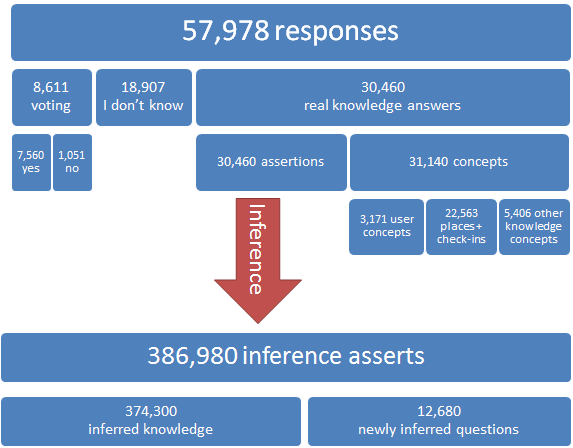
\includegraphics[width=1\textwidth]{figures/results.png}
	\caption{Graphical representation of collected answers (knowledge) and 
    distributions.}
	\label{fig:results}
\end{figure}

\begin{table}[h]
\centering
\caption{Examples of answered/asserted and inferred knowledge taken from
\emph{Curious Cat} KB.}
\label{tab:ccresultexamples}
\begin{tabular}{|c|l|l|}
	\hline
	\makecell[l]{\textbf{Type of the} \\ \textbf{collected knowledge}} & \textbf{Curious Cat Question} & \textbf{User Answer} \\
    \hline
    \textbf{User Concepts} &\makecell[l]{[automatic assert \\from registration]} & \makecell[l]{$is(User1,Person)$, \\ $name(User1,"Luka")$} \\
    \hline
    \textbf{Places + Check-ins} &\makecell[l]{[automatic assert \\from check-in \\ and Foursquare/\\Factual locations]} & \makecell[l]{$is(Place1,Restaurant)$, \\ $name(Place1,$\\"Pig'n Whistle"$)$} \\
     \hline
    \textbf{Other Concepts} &\makecell[l]{What did you order?} & \makecell[l]{Duck meat} \\
	\hline 
    \textbf{Real Knowledge 1} & Who is CEO of BMW? & Harald Kruger\\
	\hline
    \textbf{Real Knowledge 2} &\makecell[l]{What is the ticker symbol\\ of BMW?} & ABC \\
	\hline
    \textbf{voting(yes)} &\makecell[l]{Is it true that Herald Krueger\\ is the CEO of BMW company?} & yes \\
	\hline
    \textbf{voting(no)} &\makecell[l]{Is it true that ABC \\is the ticker symbol for BMW?} & no \\
	\hline
    \textbf{I don't know} &\makecell[l]{\_\_\_ and BMW are \\corporate competitors.} & I don't know \\
	\hline
    \textbf{Inferred knowledge 1} &\multicolumn{2}{l|}{$is(HeraldKrueger,Person)$} \\
	\hline
    \textbf{Inferred knowledge 2} &\multicolumn{2}{l|}{$anatomicalParts(HeraldKrueger,Hand)$} \\
	\hline
    \makecell[l]{\bfseries{Newly Inferred}\\ \bfseries{question}} &\multicolumn{2}{l|}{"What is Herald Krueger's age?"} \\
	\hline
\end{tabular}
\end{table}

While the resulting number and quality (\hl{Table XI, Table XII}) of assertions
shows that the presented approach can be successfully used for high quality KA,
we explored in more detail the contributions of specific characteristics of our
system and compare them to the baselines, to evaluate the ideas and claims
of the approach:
\begin{enumerate}
\item dada
\end{enumerate}
